\chapter{DLS}


\label{chap:dls}
Data Logging Service (DLS) is a data logging system for EtherLab. It
connects to PdServ and stores the time-series to disk.
The official documentation is available in \cite{dls_user_manual}.


\section{Install prerequesites}

The following prerequesites must be installed to compile DLS.

\subsubsection{Binary packages}
\begin{verbatim}
sudo apt install autoconf libtool libexpat1-dev    \
                 libxml2-dev libfltk1.3-dev        \
                 libfftw3-dev liburiparser-dev     \
                 protobuf-compiler libprotobuf-dev \
                 libpcre3-dev
\end{verbatim}

\subsubsection{PdCom library}
PdCom is the library to speak with PdServ. It must be downloaded and
compiled from the sources.

\noindent Download and compile PdCom library
\begin{verbatim}
cd /tmp
git clone https://gitlab.com/etherlab.org/pdcom.git
cd pdcom
git checkout 3.0.9
./bootstrap.sh
./configure --prefix=/opt/etherlab
make
\end{verbatim}

\noindent Install the PdCom library
\begin{verbatim}
sudo make install
\end{verbatim}



\section{Get DLS source code}
Download the source code with mercurial, then switch to the revision
that has been tested in this tutorial (rev 370553789444).
\begin{verbatim}
cd /tmp
git clone https://gitlab.com/etherlab.org/dls.git
cd dls
git checkout 370553789444fc6c19ae22091db00067791370ef
\end{verbatim}

\section{Compile DLS source code}

DLS uses a classic autoconf script to generate the Makefile.
\begin{verbatim}
cd /tmp/dls
./bootstrap.sh
./configure --prefix=/opt/etherlab
make
\end{verbatim}


\section{Install DLS programs}
The programs are installed in \texttt{/opt/etherlab} \\

\begin{verbatim}
sudo make -C /tmp/dls install
sudo ldconfig
\end{verbatim}

\subsubsection{Create system account}
Create a system account \texttt{dls}

\begin{verbatim}
sudo useradd -s /usr/sbin/nologin -r dls
\end{verbatim}


\subsubsection{Create data directories}

Create a directory (\texttt{/home/dls/data}) to store recorded data.
\begin{verbatim}
sudo install -d -o dls -g dls /home/dls/data
\end{verbatim} 


\section{Manage acquisition with dls\_ctl }

The acquisition are managed with \texttt{dls\_ctl}.

\begin{verbatim}
sudo -i
export PATH=/opt/etherlab/bin:$PATH
dls_ctl -d /home/dls/data
\end{verbatim}

\subsubsection{Initialize the data directory}
The main window appears. The program asks if the data directory
  shall be initialized. Answer YES.

\begin{center}
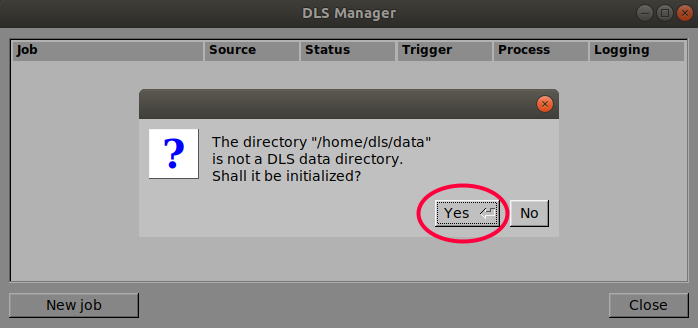
\includegraphics[width=\textwidth]{genpicts/dls_ctl-00.eps}
\end{center}

\subsubsection{Start the acquisition daemon}
The program asks if the acquisition daemon
  shall be started. Answer YES.

\begin{center}
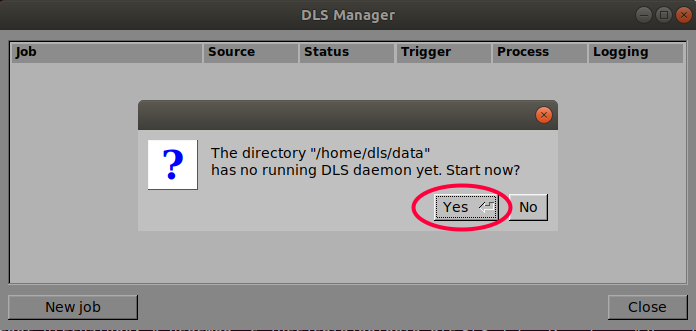
\includegraphics[width=\textwidth]{genpicts/dls_ctl-01.eps}
\end{center}

\noindent In the console, a message shows that the dls daemon is now running.

\begin{verbatim}
dls_ctl 1.4.0-rc2 revision 51dc3443178a
DLS data directory "/home/dls/data"
dlsd 1.4.0-rc2 revision 51dc3443178a
Using dls directory "/home/dls/data"
DLS running with PID 26307 [daemon]
\end{verbatim}


\subsubsection{Configure acquisition}

\noindent Click \textit{New job} to create a new acquisition job
\begin{center}
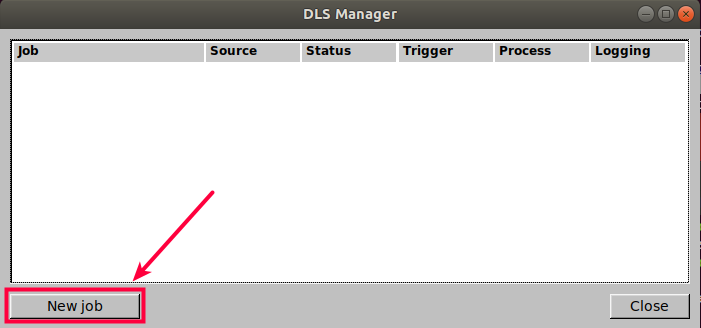
\includegraphics[width=\textwidth]{genpicts/dls_ctl-02.eps}
\end{center}


\noindent Fill the form with the job properties. Warning: unlike the others,
the field \textit{Source} cannot be modify later. therefore it must be
enter correctly at the first time.

\begin{center}
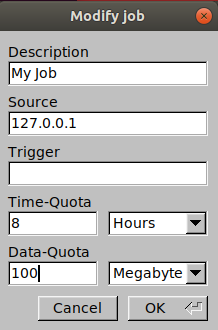
\includegraphics[width=0.35\textwidth]{genpicts/dls_ctl-03.eps}
\end{center}

\noindent The new job appears in the list, double-click on it
to edit the channels.

\begin{center}
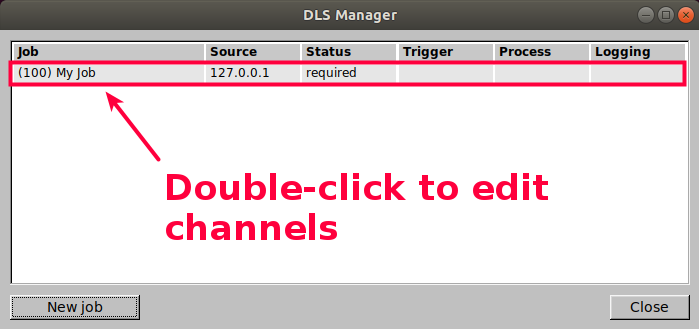
\includegraphics[width=\textwidth]{genpicts/dls_ctl-04.eps}
\end{center}

\noindent Click on \textit{Add channels...}
\begin{center}
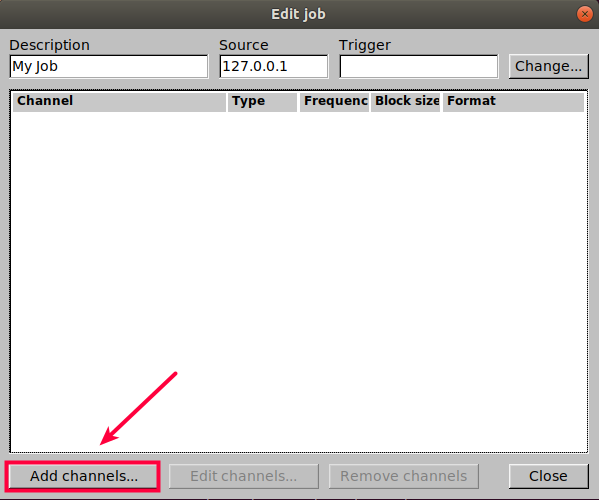
\includegraphics[width=0.75\textwidth]{genpicts/dls_ctl-05.eps}
\end{center}

\noindent Select channel \textit{/s1/c}
\begin{center}
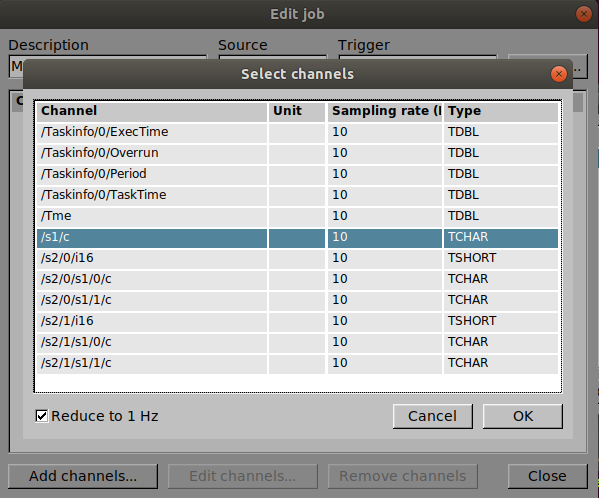
\includegraphics[width=0.75\textwidth]{genpicts/dls_ctl-06.eps}
\end{center}

\noindent Close the job window.
\begin{center}
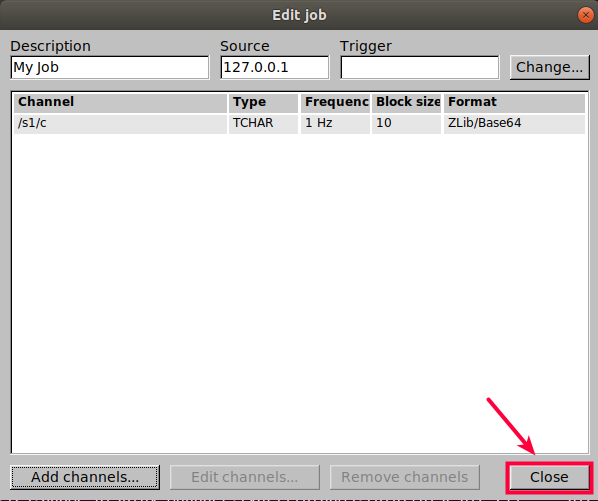
\includegraphics[width=0.75\textwidth]{genpicts/dls_ctl-07.eps}
\end{center}

\noindent Click on the button \textit{Start}
\begin{center}
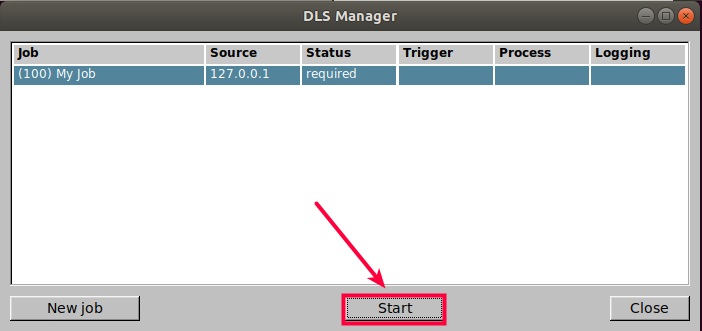
\includegraphics[width=\textwidth]{genpicts/dls_ctl-08.eps}
\end{center}

\noindent The aquisition is running.
\begin{center}
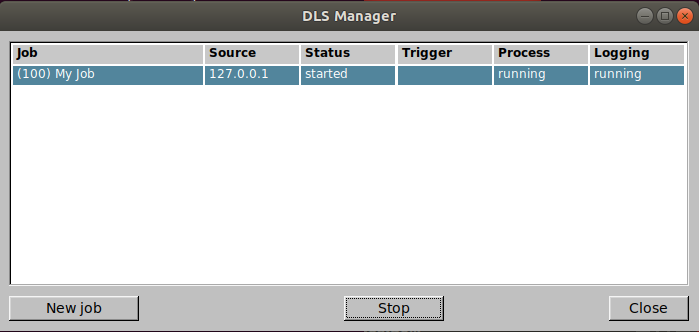
\includegraphics[width=\textwidth]{genpicts/dls_ctl-09.eps}
\end{center}




\section{Plot channels with dls\_view }

\texttt{dls\_view} is the legacy viewer for DLS.
The newer viewer (\texttt{dlsgui}) is explained in section \ref{chap:dlsgui}.


\subsubsection{Run dls\_view}

Unlike \texttt{dlsgui}, \texttt{dls\_view} needs filesystem access to the
recorded data.

\begin{verbatim}
sudo -i
export PATH=/opt/etherlab/bin:$PATH
dls_view -d /home/dls/data
\end{verbatim}


\noindent Select the acquisition job to display

\begin{center}
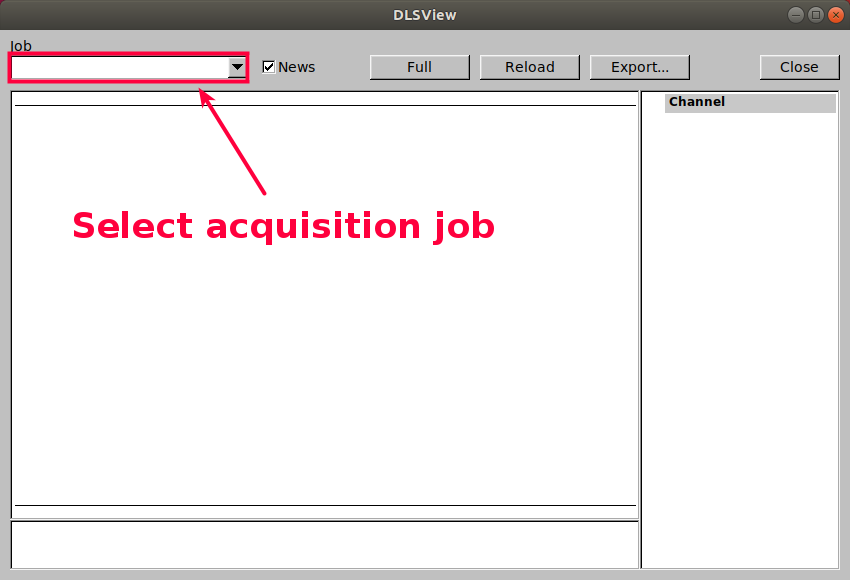
\includegraphics[width=0.9\textwidth]{genpicts/dls_view-00.eps}
\end{center}


\noindent Select the channel to display
\begin{center}
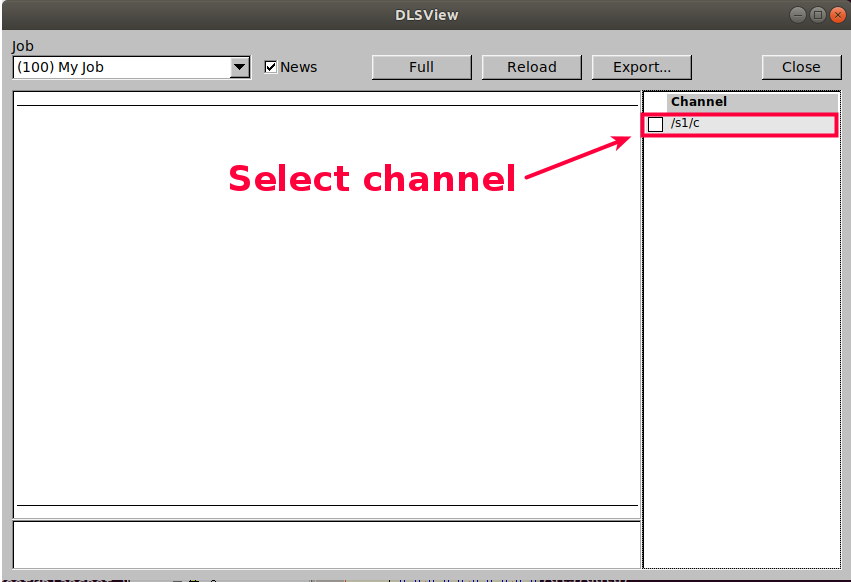
\includegraphics[width=0.9\textwidth]{genpicts/dls_view-01.eps}
\end{center}


\noindent The plot appears as a green rectangle because but the lines
are overmuch condensed.

\begin{center}
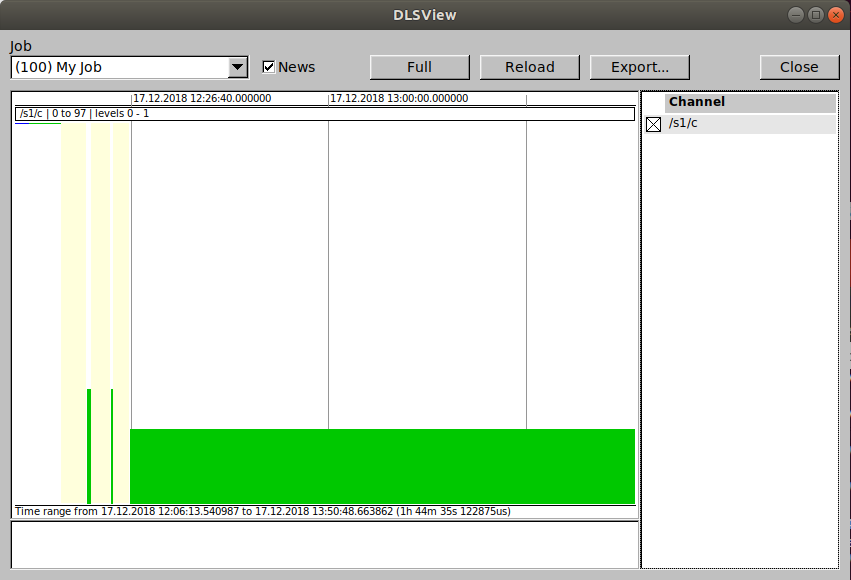
\includegraphics[width=0.9\textwidth]{genpicts/dls_view-02.eps}
\end{center}


\noindent Draw a rectangle in the viewing area to zoom in, click on
the viewing area to zoom out. See \cite{dls_user_manual} for the
complete description of the user interface.

\begin{center}
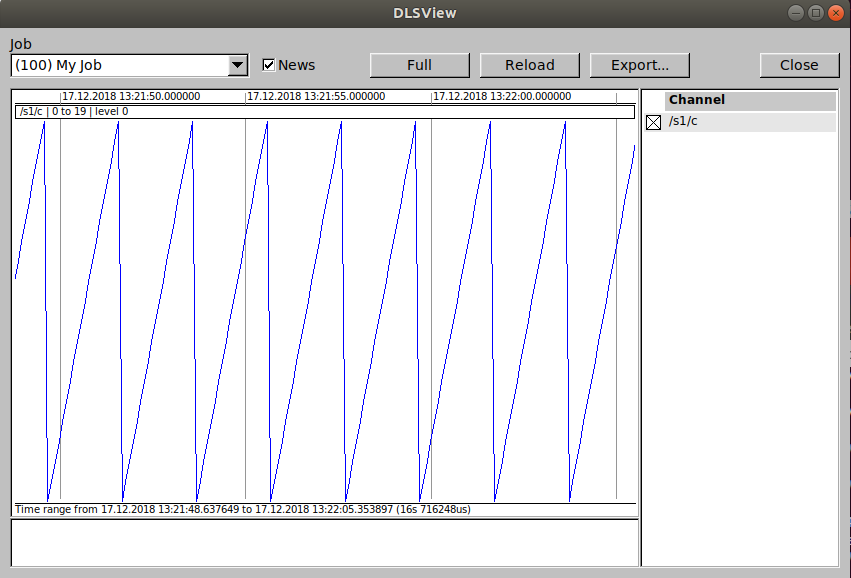
\includegraphics[width=0.9\textwidth]{genpicts/dls_view-03.eps}
\end{center}
